\documentclass[12pt, letterpaper]{article}
\usepackage{graphicx}
\usepackage{fancyhdr}
\graphicspath{{.github/workflows/Images/}}
\usepackage{tikz} 
\usepackage{tocloft}
\renewcommand{\cftsecleader}{\cftdotfill{\cftdotsep}} 

\title{Computer Workshop\\ Final Assignment : All Together}
\author{Kasra Khalaj}
\date{Due: 7 Bahman, 1402}

\begin{document}
\pagenumbering{gobble}
\maketitle
\newpage
\pagenumbering{arabic}
\large

\tableofcontents
\section{Git and GitHub}
\subsection{ Repository Initialization and Commits}
Firstly i created a normal folder and initialized a Git repository using the git init command in my powershell, after creating a new repo on GitHub, i copied the link in the Code tab and used git clone <url> in my powershell in the folder which a git repo was initialized using git init. then i made a .github folder and then in it a workflow folder to copy the main.yml file in it, then i made a 
 simple latex doc named main.tex for the very start, then i simply used the command git add . And this is optional now in some way but in order to practice tags i used git tag 1.0.0. and then git commit -m "Added the workflow and main.tex files and folders". Then i simply pushed the origin main to update my Github repo, everything else is going to be like this in some way.
 \subsection{GitHub Actions for LaTeX Compilation}
 I've actually answered to this in my previous response. Everything is done by the main.yml that we have in our workflow folder in some way. The workflow has some particular configuration to make a certain .tex file to a .pdf file. The challenge i encountered was the fact that if i want to make releases of main.pdf, i have to use the tag when pushing too like this => "git push origin 1.9.8", when using this command the release version 1.9.8 will be deplying the main.pdf file in the actions/workflows, when it's deployed, the file is easily downloadable. This is amazing. GitHub vaghean fogholadas aslan ashnayiati nadashtam, hanuzam kheili kheili kam daram vali be lotfe shoma ziad shod etelaatam mamnonam kheili kelase khubi bud.
\section{ Exploration Tasks}
\subsection{Vim Advanced Features}
 Vimscript:

Firstly, one fact which can be very interesting is to build costume commands and functions with vimscript. \textbf{Vimscript} is the scripting language built into Vim, which users can automate tasks, create custom commands, and customize Vim's behavior to suit their workflow.
Users can also define custom functions, mappings, commands and autocommands using Vimscript too!
To create a Vimscript function, use the function keyword followed by the function name and the function body enclosed in curly braces. For example: \\
function! MyFunction() \\
  " Function body here .............. " \\ 
endfunction \\
This is an example of how to make a vimscript cmmand ourselves.
Secondly, Vim includes a built-in tool called \textbf{Vimdiff} for performing file comparisons and merges.
Users can compare two or three files side by side, highlighting the differences between them.
Vimdiff provides powerful editing commands for merging changes from one file to another, resolving conflicts, and navigating between differences.
And finaly, vim alse allows users to save and restore editing sessions, preserving the state of open files, window layouts, and other settings.
Users can save a session using the \textbf{:mksession} command and restore it later using the -S option when launching Vim or by running :source on the session file.
Session management plugins like vim-session provide additional features for organizing and managing multiple sessions.
\subsection{ Memory profiling}
\subsubsection{Memory Leak}
In general, Memory leaks occur when a program allocates memory dynamically via using malloc and pointers mainly, but then people fail to release that memory when it's no longer needed with using free(folan). This can lead to crashes and stuff.
\subsubsection{Memory profilers}
Valgrind's main feature for memory leak detection is its Memcheck tool. Memcheck performs dynamic analysis of a program's memory usage during runtime, tracking all memory allocations and deallocations.
When the program terminates, Memcheck generates a report highlighting any memory blocks that were \textbf{allocated} but not deallocated, indicating potential memory leaks.
\subsection{GNU/Linux Bash Scripting}
\subsubsection{fzf}
In fuzzy searching, a similarity score is calculated between the search query and each potential match in the target text. This score is based on various factors such as character similarity, edit distance, and token similarity. The search algorithm then ranks the matches based on their similarity scores, returning the most relevant results to the user which is the exact same thing that fzf command does.
Upon execution, fzf displays a searchable list of files and directories from the output of ls. Users can then type a search query to perform fuzzy searching and narrow down the list of items. Pressing Enter selects the highlighted item, which can then be further processed or acted upon by subsequent commands in the pipeline.



\section{Git and FOSS}

\subsubsection{README.MD}
Done!
\subsection{Issues}

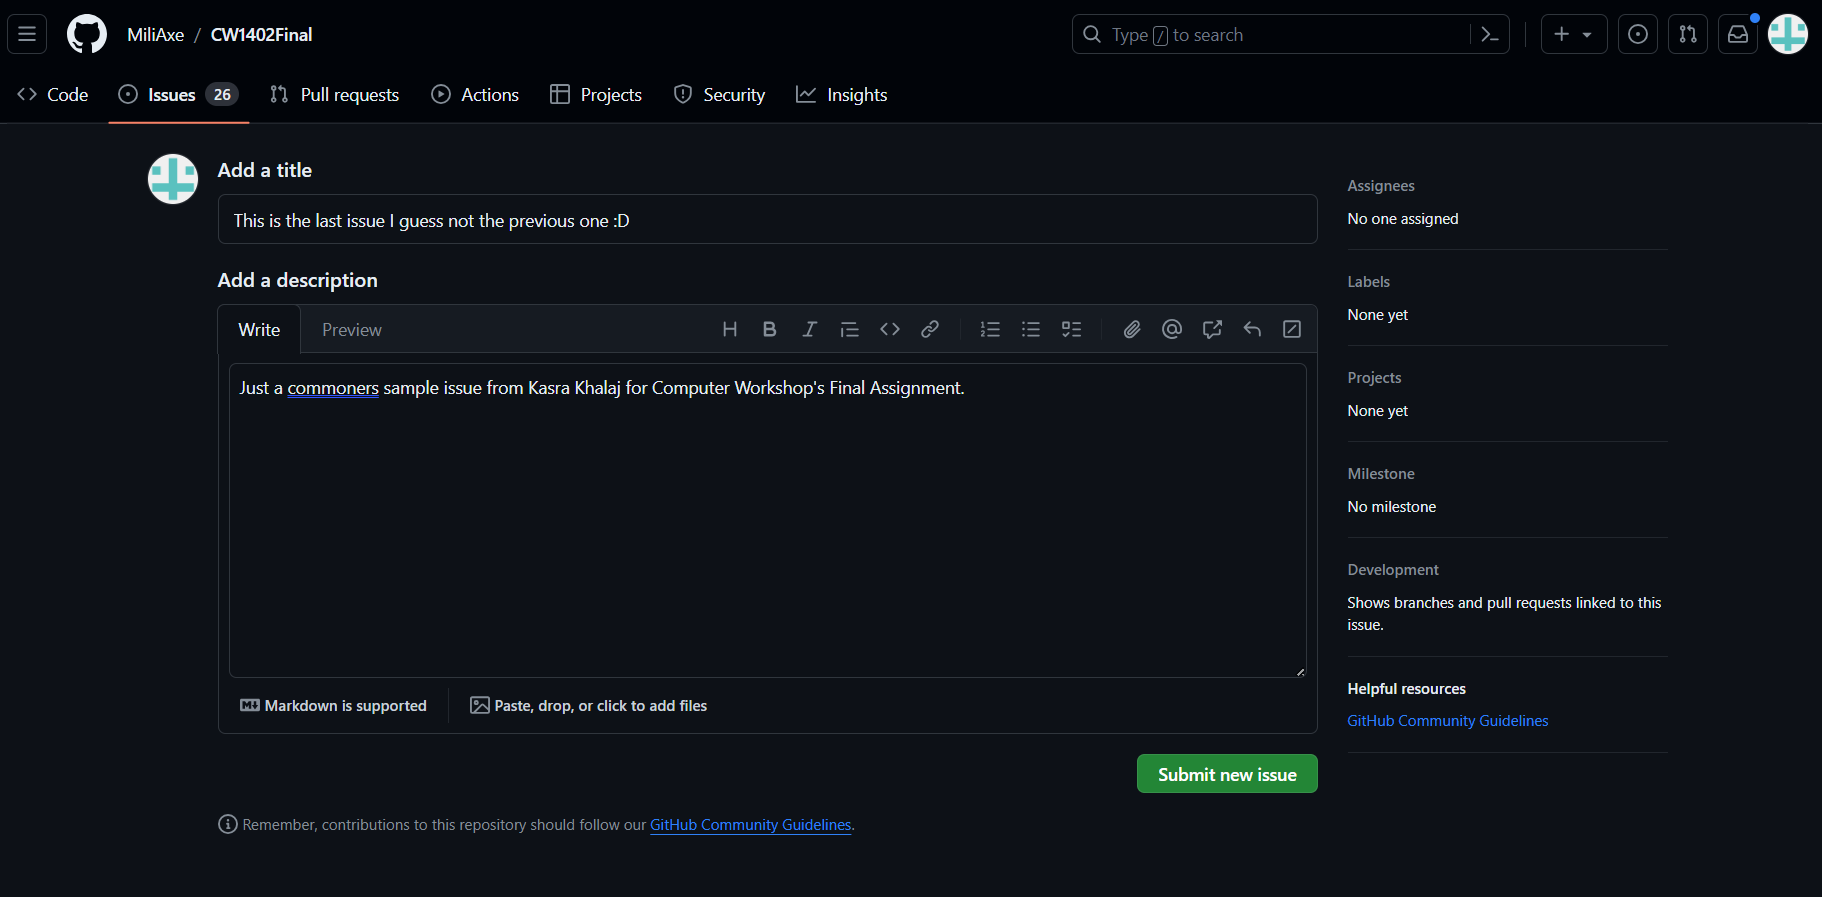
\includegraphics[width=15cm, height=10cm]{Images/SampleIssue.png}


\end{document}